\begin{definitionbox}{Definition --- Metric Space}
\begin{definition}[Metric Space]\label{def:metric-space}
A \emph{metric space} is a pair \((X,d)\), where \(X\) is a set and \(d\) is
a metric on \(X\).
\end{definition}
\end{definitionbox}

\begin{remark*}[Standard quantified statement]
\[
(X,d)
\quad\text{with}\quad
d \text{ a metric on } X.
\]
\end{remark*}

\begin{remark*}[Interpretation]
A metric space is a set equipped with a chosen metric.  The set supplies the
points, and the metric supplies the distance structure on those points.
\end{remark*}

\begin{remark*}[Historical note]
This definition is modeled on Definition~1.1.1 of
{\'O} Searc{\'o}id's \emph{Metric Spaces} \cite{OSearcoidMetricSpaces}.
\end{remark*}

\LeanFormalizes{def:metric-space}{lra-lean}{LRA.VolumeIV.MetricSpaces.Foundations.MetricSpace}{MetricSpaceDefinition}{statement}

\begin{dependencies}
\begin{itemize}
  \item \hyperref[def:metric-on-set]{Definition: Metric}
\end{itemize}
\end{dependencies}

\begin{theorembox}{Theorem}
\begin{theorem}[Rearrangement of the Triangle Inequality]
\label{thm:metric-rearranged-triangle-inequality}
Let \((X,d)\) be a metric space.  For all \(a,b,c\in X\),
\[
  \bigl|d(a,b)-d(b,c)\bigr|\leq d(a,c).
\]

\smallskip
\noindent
\hyperref[prf:metric-rearranged-triangle-inequality]{\textit{Go to proof.}}
\end{theorem}
\end{theorembox}

\begin{remark*}[Standard quantified statement]
\[
\forall a,b,c\in X{:}\;
\bigl|d(a,b)-d(b,c)\bigr|\leq d(a,c).
\]
\end{remark*}

\begin{remark*}[Predicate reading]
\[
\bigl|d(a,b)-d(b,c)\bigr|\leq d(a,c)
\]
means that the two distances from \(b\) to \(a\) and from \(b\) to \(c\)
differ by at most the distance from \(a\) to \(c\).
\end{remark*}

\begin{remark*}[Interpretation]
In a metric space, the distances from \(b\) to \(a\) and from \(b\) to \(c\)
cannot differ by more than the distance between \(a\) and \(c\).  This is the
triangle inequality rearranged so that one distance controls the difference
between two others.
\end{remark*}

\begin{remark*}[Historical note]
This theorem is modeled on Theorem~1.1.2 of
{\'O} Searc{\'o}id's \emph{Metric Spaces} \cite{OSearcoidMetricSpaces}.
\end{remark*}

\LeanFormalizes{thm:metric-rearranged-triangle-inequality}{lra-lean}{LRA.VolumeIV.MetricSpaces.Foundations.MetricSpace}{rearrangement_of_triangle_inequality}{statement}

\begin{dependencies}
\begin{itemize}
  \item \hyperref[def:metric-space]{Definition: Metric Space}
\end{itemize}
\end{dependencies}

\begin{definitionbox}{Definition --- Real-Line Euclidean Metric Space}
\begin{definition}[Real-Line Euclidean Metric Space]
\label{def:real-line-euclidean-metric-space}
The \emph{real-line Euclidean metric space} is
\[
  (\mathbb{R},d_{\mathbb{R}}),
\]
where \(d_{\mathbb{R}}(x,y)=|x-y|\).
\end{definition}
\end{definitionbox}

\begin{remark*}[Standard quantified statement]
\[
\mathsf{MetricSpace}(\mathbb{R},d_{\mathbb{R}}).
\]
\end{remark*}

\begin{remark*}[Interpretation]
This is the usual real line viewed as a metric space by absolute-value
distance.
\end{remark*}

\begin{dependencies}
\begin{itemize}
  \item \hyperref[def:real-line-euclidean-distance]{Definition: Euclidean Distance on \(\mathbb{R}\)}
  \item \hyperref[def:metric-space]{Definition: Metric Space}
  \item \hyperref[prop:real-line-euclidean-distance-metric]{Proposition: The Real-Line Euclidean Distance is a Metric}
\end{itemize}
\end{dependencies}

\begin{propositionbox}{Proposition}
\begin{proposition}[The Real Line is a Metric Space]
\label{prop:real-line-euclidean-metric-space}
The pair \((\mathbb{R},d_{\mathbb{R}})\) is a metric space.

\smallskip
\noindent
\hyperref[prf:real-line-euclidean-metric-space]{\textit{Go to proof.}}
\end{proposition}
\end{propositionbox}

\begin{remark*}[Standard quantified statement]
\[
  \mathsf{MetricSpace}(\mathbb{R},d_{\mathbb{R}}).
\]
\end{remark*}

\begin{remark*}[Interpretation]
The metric-space structure follows from the real-line Euclidean distance satisfying the metric axioms.
\end{remark*}

\begin{dependencies}
\begin{itemize}
  \item \hyperref[def:real-line-euclidean-metric-space]{Definition: Real-Line Euclidean Metric Space}
  \item \hyperref[def:metric-space]{Definition: Metric Space}
  \item \hyperref[prop:real-line-euclidean-distance-metric]{Proposition: The Real-Line Euclidean Distance is a Metric}
\end{itemize}
\end{dependencies}

\begin{definitionbox}{Definition --- Euclidean Metric Space}
\begin{definition}[Euclidean Metric Space]\label{def:euclidean-metric-space}
For \(n\in\mathbb{N}\), the \emph{standard Euclidean metric space} is
\[
  (\mathbb{R}^n,d_2),
\]
where \(d_2\) is the Euclidean metric on \(\mathbb{R}^n\).
\end{definition}
\end{definitionbox}

\begin{remark*}[Standard quantified statement]
\[
n\in\mathbb{N}
\Longrightarrow
\operatorname{MetricSpace}(\mathbb{R}^n,d_2).
\]
\end{remark*}

\begin{remark*}[Interpretation]
The Euclidean metric space is the standard finite-dimensional distance model:
points are coordinate vectors, and distance is ordinary straight-line length.
\end{remark*}

\begin{dependencies}
\begin{itemize}
  \item \hyperref[def:metric-space]{Definition: Metric Space}
  \item \hyperref[def:euclidean-space]{Definition: Euclidean Space}
  \item \hyperref[def:euclidean-distance-rn]{Definition: Euclidean Distance on \(\mathbb{R}^n\)}
  \item \hyperref[cor:euclidean-metric]{Corollary: Euclidean Metric}
\end{itemize}
\end{dependencies}

\begin{corollarybox}{Corollary}
\begin{corollary}[Euclidean Metric]\label{cor:euclidean-metric}
For every \(x,y\in\mathbb{R}^n\), define
\[
  d_2(x,y):=\sqrt{|x_1-y_1|^2+\cdots+|x_n-y_n|^2}.
\]
Then \((\mathbb{R}^n,d_2)\) is a metric space.

\smallskip
\noindent
\hyperref[prf:euclidean-metric]{\textit{Go to proof.}}
\end{corollary}
\end{corollarybox}

\begin{remark*}[Standard quantified statement]
\[
\operatorname{IsMetric}(\mathbb{R}^n,d_2).
\]
\end{remark*}

\begin{remark*}[Predicate reading]
\[
\operatorname{IsMetric}(\mathbb{R}^n,d_2)
\]
means that \(d_2\) gives the standard Euclidean metric-space structure on
\(\mathbb{R}^n\).
\end{remark*}

\begin{remark*}[Interpretation]
This records the standard Euclidean metric-space structure on
\(\mathbb{R}^n\).
\end{remark*}

\begin{dependencies}
\begin{itemize}
  \item \hyperref[def:metric-space]{Definition: Metric Space}
  \item \hyperref[def:euclidean-distance-rn]{Definition: Euclidean Distance on \(\mathbb{R}^n\)}
  \item \hyperref[cor:minkowski-inequality-rn]{Corollary: Minkowski's Inequality}
\end{itemize}
\end{dependencies}

\begin{definitionbox}{Definition --- Taxicab Metric Space}
\begin{definition}[Taxicab Metric Space]\label{def:taxicab-metric-space}
For \(n\in\mathbb{N}\), the \emph{taxicab metric space} is
\[
  (\mathbb{R}^n,d_1),
\]
where \(d_1\) is the taxicab metric on \(\mathbb{R}^n\).
\end{definition}
\end{definitionbox}

\begin{remark*}[Standard quantified statement]
\[
n\in\mathbb{N}
\Longrightarrow
\operatorname{MetricSpace}(\mathbb{R}^n,d_1).
\]
\end{remark*}

\begin{remark*}[Interpretation]
The taxicab metric space has the same underlying set as Euclidean space, but
distance is measured by summing coordinatewise displacements.
\end{remark*}

\begin{dependencies}
\begin{itemize}
  \item \hyperref[def:metric-space]{Definition: Metric Space}
  \item \hyperref[def:taxicab-metric-rn]{Definition: Taxicab Metric}
  \item \hyperref[prop:taxicab-metric-rn]{Proposition: Taxicab Metric}
\end{itemize}
\end{dependencies}

\begin{propositionbox}{Proposition}
\begin{proposition}[The Taxicab Metric Space is a Metric Space]
\label{prop:taxicab-metric-space-instance}
For every \(n\in\mathbb{N}\), the pair \((\mathbb{R}^n,d_1)\) is a metric space.

\smallskip
\noindent
\hyperref[prf:taxicab-metric-space-instance]{\textit{Go to proof.}}
\end{proposition}
\end{propositionbox}

\begin{remark*}[Standard quantified statement]
\[
  n\in\mathbb{N}\Longrightarrow\mathsf{MetricSpace}(\mathbb{R}^n,d_1).
\]
\end{remark*}

\begin{remark*}[Interpretation]
This packages the taxicab metric as a metric-space structure on \(\mathbb{R}^n\).
\end{remark*}

\begin{dependencies}
\begin{itemize}
  \item \hyperref[def:metric-space]{Definition: Metric Space}
  \item \hyperref[def:taxicab-metric-space]{Definition: Taxicab Metric Space}
  \item \hyperref[prop:taxicab-metric-rn]{Proposition: Taxicab Metric}
\end{itemize}
\end{dependencies}

\begin{definitionbox}{Definition --- \(p\)-Metric Space}
\begin{definition}[\(p\)-Metric Space]\label{def:lp-metric-space}
Let \(1\leq p<\infty\) and let \(n\in\mathbb{N}\).  The \emph{\(p\)-metric
space} is
\[
  (\mathbb{R}^n,d_p),
\]
where \(d_p\) is the \(p\)-metric on \(\mathbb{R}^n\).
\end{definition}
\end{definitionbox}

\begin{remark*}[Standard quantified statement]
\[
1\leq p<\infty,\; n\in\mathbb{N}
\Longrightarrow
\operatorname{MetricSpace}(\mathbb{R}^n,d_p).
\]
\end{remark*}

\begin{remark*}[Interpretation]
The \(p\)-metric spaces form a family of finite-dimensional metric spaces on
the same coordinate set, with different rules for turning coordinate
displacements into distance.
\end{remark*}

\begin{figure}[htbp]
\centering
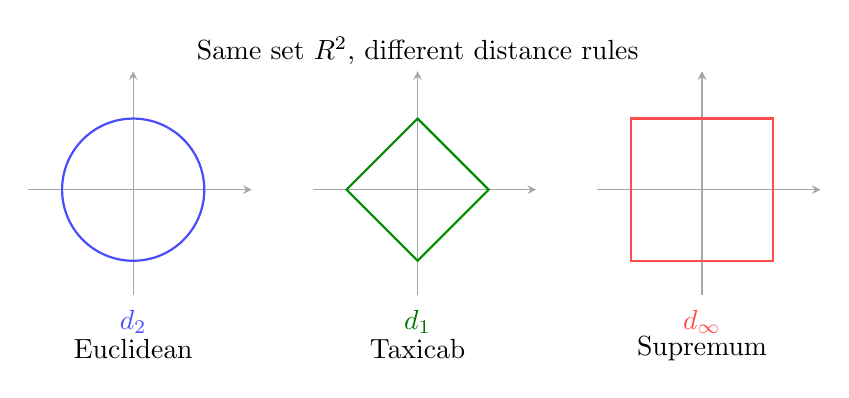
\begin{tikzpicture}[scale=0.86,>=stealth]
  \draw[->,gray!70] (-1.55,0) -- (1.75,0);
  \draw[->,gray!70] (0,-1.55) -- (0,1.75);
  \draw[blue!70,thick] (0,0) circle (1.05);
  \node[blue!70] at (0,-1.95) {\(d_2\)};
  \node at (0,-2.35) {Euclidean};

  \begin{scope}[xshift=4.2cm]
    \draw[->,gray!70] (-1.55,0) -- (1.75,0);
    \draw[->,gray!70] (0,-1.55) -- (0,1.75);
    \draw[green!55!black,thick]
      (0,1.05) -- (1.05,0) -- (0,-1.05) -- (-1.05,0) -- cycle;
    \node[green!45!black] at (0,-1.95) {\(d_1\)};
    \node at (0,-2.35) {Taxicab};
  \end{scope}

  \begin{scope}[xshift=8.4cm]
    \draw[->,gray!70] (-1.55,0) -- (1.75,0);
    \draw[->,gray!70] (0,-1.55) -- (0,1.75);
    \draw[red!70,thick] (-1.05,-1.05) rectangle (1.05,1.05);
    \node[red!70] at (0,-1.95) {\(d_\infty\)};
    \node at (0,-2.35) {Supremum};
  \end{scope}

  \node[align=center] at (4.2,2.05)
    {Same set \(\mathbb{R}^2\), different distance rules};
\end{tikzpicture}

\caption{Different metrics on the same underlying set can produce different
metric shapes.  The unit ball in \(\mathbb{R}^2\) changes when distance is
measured by \(d_2\), \(d_1\), or \(d_\infty\).}
\label{fig:metric-unit-balls-r2}
\end{figure}

\begin{dependencies}
\begin{itemize}
  \item \hyperref[def:metric-space]{Definition: Metric Space}
  \item \hyperref[def:lp-metric-rn]{Definition: \(p\)-Metric on \(\mathbb{R}^n\)}
  \item \hyperref[thm:lp-metric-rn]{Theorem: \(d_p\) is a Metric}
\end{itemize}
\end{dependencies}

\begin{propositionbox}{Proposition}
\begin{proposition}[The \(p\)-Metric Space is a Metric Space]
\label{prop:lp-metric-space-instance}
For every \(1\leq p<\infty\) and every \(n\in\mathbb{N}\), the pair \((\mathbb{R}^n,d_p)\) is a metric space.

\smallskip
\noindent
\hyperref[prf:lp-metric-space-instance]{\textit{Go to proof.}}
\end{proposition}
\end{propositionbox}

\begin{remark*}[Standard quantified statement]
\[
  1\leq p<\infty,\; n\in\mathbb{N}\Longrightarrow\mathsf{MetricSpace}(\mathbb{R}^n,d_p).
\]
\end{remark*}

\begin{remark*}[Interpretation]
This packages each finite-dimensional \(p\)-metric as a metric-space structure.
\end{remark*}

\begin{dependencies}
\begin{itemize}
  \item \hyperref[def:metric-space]{Definition: Metric Space}
  \item \hyperref[def:lp-metric-space]{Definition: \(p\)-Metric Space}
  \item \hyperref[thm:lp-metric-rn]{Theorem: \(d_p\) is a Metric}
\end{itemize}
\end{dependencies}

\begin{definitionbox}{Definition --- Complex Metric Space}
\begin{definition}[Complex Metric Space]\label{def:complex-metric-space}
The \emph{complex metric space} is
\[
  (\mathbb{C},d_{\mathbb{C}}),
\]
where \(d_{\mathbb{C}}\) is the usual Euclidean distance on the complex plane.
\end{definition}
\end{definitionbox}

\begin{remark*}[Standard quantified statement]
\[
\operatorname{MetricSpace}(\mathbb{C},d_{\mathbb{C}}).
\]
\end{remark*}

\begin{remark*}[Interpretation]
The complex metric space treats complex numbers as points in the Euclidean
plane, while retaining the notation and algebra of \(\mathbb{C}\).
\end{remark*}

\begin{dependencies}
\begin{itemize}
  \item \hyperref[def:complex-metric]{Definition: Complex Metric}
  \item \hyperref[def:metric-space]{Definition: Metric Space}
  \item \hyperref[prop:complex-plane-metric-space]{Proposition: The Complex Plane is a Metric Space}
\end{itemize}
\end{dependencies}

\begin{propositionbox}{Proposition}
\begin{proposition}[The Complex Plane is a Metric Space]
\label{prop:complex-plane-metric-space}
The pair \((\mathbb{C},d_{\mathbb{C}})\) is a metric space.

\smallskip
\noindent
\hyperref[prf:complex-plane-metric-space]{\textit{Go to proof.}}
\end{proposition}
\end{propositionbox}

\begin{remark*}[Standard quantified statement]
\[
  \operatorname{IsMetric}(\mathbb{C},d_{\mathbb{C}}).
\]
\end{remark*}

\begin{remark*}[Predicate reading]
\[
\operatorname{IsMetric}(\mathbb{C},d_{\mathbb{C}})
\]
means that modulus distance is a metric on the complex plane.
\end{remark*}

\begin{remark*}[Interpretation]
The metric on \(\mathbb{C}\) is inherited from the Euclidean plane.
\end{remark*}

\begin{dependencies}
\begin{itemize}
  \item \hyperref[def:complex-metric]{Definition: Complex Metric}
  \item \hyperref[def:metric-space]{Definition: Metric Space}
  \item \hyperref[cor:euclidean-metric]{Corollary: Euclidean Metric}
\end{itemize}
\end{dependencies}

\begin{definitionbox}{Definition --- Real Circle Chord Metric Space}
\begin{definition}[Real Circle Chord Metric Space]
\label{def:real-circle-chord-metric-space}
The \emph{real circle chord metric space} is
\[
  (S^1_{\mathbb{R}},d_{\mathrm{chord},\mathbb{R}}),
\]
where \(d_{\mathrm{chord},\mathbb{R}}\) is the real circle chord metric.
\end{definition}
\end{definitionbox}

\begin{remark*}[Standard quantified statement]
\[
\mathsf{MetricSpace}(S^1_{\mathbb{R}},d_{\mathrm{chord},\mathbb{R}}).
\]
\end{remark*}

\begin{remark*}[Interpretation]
The real unit circle becomes a metric space by measuring straight-line chord
distance between points.
\end{remark*}

\begin{dependencies}
\begin{itemize}
  \item \hyperref[def:real-circle-chord-metric]{Definition: Real Circle Chord Metric}
  \item \hyperref[def:metric-space]{Definition: Metric Space}
  \item \hyperref[prop:real-circle-chord-metric]{Proposition: The Real Circle Chord Distance is a Metric}
\end{itemize}
\end{dependencies}

\begin{propositionbox}{Proposition}
\begin{proposition}[The Real Circle Chord Metric Space is a Metric Space]
\label{prop:real-circle-chord-metric-space}
The pair \((S^1_{\mathbb{R}},d_{\mathrm{chord},\mathbb{R}})\) is a metric space.

\smallskip
\noindent
\hyperref[prf:real-circle-chord-metric-space]{\textit{Go to proof.}}
\end{proposition}
\end{propositionbox}

\begin{remark*}[Standard quantified statement]
\[
  \mathsf{MetricSpace}(S^1_{\mathbb{R}},d_{\mathrm{chord},\mathbb{R}}).
\]
\end{remark*}

\begin{remark*}[Interpretation]
This records the metric-space structure induced by chord distance on the real unit circle.
\end{remark*}

\begin{dependencies}
\begin{itemize}
  \item \hyperref[def:real-circle-chord-metric-space]{Definition: Real Circle Chord Metric Space}
  \item \hyperref[def:metric-space]{Definition: Metric Space}
  \item \hyperref[prop:real-circle-chord-metric]{Proposition: The Real Circle Chord Distance is a Metric}
\end{itemize}
\end{dependencies}

\begin{definitionbox}{Definition --- Complex Circle Chord Metric Space}
\begin{definition}[Complex Circle Chord Metric Space]
\label{def:complex-circle-chord-metric-space}
The \emph{complex circle chord metric space} is
\[
  (S^1_{\mathbb{C}},d_{\mathrm{chord},\mathbb{C}}),
\]
where \(d_{\mathrm{chord},\mathbb{C}}\) is the complex circle chord metric.
\end{definition}
\end{definitionbox}

\begin{remark*}[Standard quantified statement]
\[
\mathsf{MetricSpace}(S^1_{\mathbb{C}},d_{\mathrm{chord},\mathbb{C}}).
\]
\end{remark*}

\begin{remark*}[Interpretation]
The complex unit circle becomes a metric space by restricting complex modulus
distance to points of modulus one.
\end{remark*}

\begin{dependencies}
\begin{itemize}
  \item \hyperref[def:complex-circle-chord-metric]{Definition: Complex Circle Chord Metric}
  \item \hyperref[def:metric-space]{Definition: Metric Space}
  \item \hyperref[prop:complex-circle-chord-metric]{Proposition: The Complex Circle Admits the Chord Metric}
\end{itemize}
\end{dependencies}

\begin{propositionbox}{Proposition}
\begin{proposition}[The Complex Circle Chord Metric Space is a Metric Space]
\label{prop:complex-circle-chord-metric-space}
The pair \((S^1_{\mathbb{C}},d_{\mathrm{chord},\mathbb{C}})\) is a metric space.

\smallskip
\noindent
\hyperref[prf:complex-circle-chord-metric-space]{\textit{Go to proof.}}
\end{proposition}
\end{propositionbox}

\begin{remark*}[Standard quantified statement]
\[
  \mathsf{MetricSpace}(S^1_{\mathbb{C}},d_{\mathrm{chord},\mathbb{C}}).
\]
\end{remark*}

\begin{remark*}[Interpretation]
This records the metric-space structure induced by chord distance on the complex unit circle.
\end{remark*}

\begin{dependencies}
\begin{itemize}
  \item \hyperref[def:complex-circle-chord-metric-space]{Definition: Complex Circle Chord Metric Space}
  \item \hyperref[def:metric-space]{Definition: Metric Space}
  \item \hyperref[prop:complex-circle-chord-metric]{Proposition: The Complex Circle Admits the Chord Metric}
\end{itemize}
\end{dependencies}

\begin{definitionbox}{Definition --- Bounded Sequence Metric Space}
\begin{definition}[Bounded Sequence Metric Space]
\label{def:bounded-sequence-metric-space}
The \emph{bounded sequence metric space} is
\[
  (\ell^\infty(\mathbb{R}),d_\infty),
\]
where \(\ell^\infty(\mathbb{R})\) is the set of bounded real sequences and
\(d_\infty\) is the supremum metric.
\end{definition}
\end{definitionbox}

\begin{remark*}[Standard quantified statement]
\[
\operatorname{MetricSpace}(\ell^\infty(\mathbb{R}),d_\infty).
\]
\end{remark*}

\begin{remark*}[Interpretation]
The bounded sequence metric space is an infinite-dimensional example.  Its
distance measures the largest coordinatewise discrepancy between two bounded
real sequences.
\end{remark*}

\begin{dependencies}
\begin{itemize}
  \item \hyperref[def:metric-space]{Definition: Metric Space}
  \item \hyperref[def:bounded-real-sequence-space]{Definition: Supremum Metric on Bounded Real Sequences}
  \item \hyperref[prop:bounded-real-sequence-space-sup-metric]{Proposition: Supremum Metric on Bounded Sequences}
\end{itemize}
\end{dependencies}

\begin{propositionbox}{Proposition}
\begin{proposition}[The Bounded Sequence Metric Space is a Metric Space]
\label{prop:bounded-sequence-metric-space}
The pair \((\ell^\infty(\mathbb{R}),d_\infty)\) is a metric space.

\smallskip
\noindent
\hyperref[prf:bounded-sequence-metric-space]{\textit{Go to proof.}}
\end{proposition}
\end{propositionbox}

\begin{remark*}[Standard quantified statement]
\[
  \mathsf{MetricSpace}(\ell^\infty(\mathbb{R}),d_\infty).
\]
\end{remark*}

\begin{remark*}[Interpretation]
This packages the supremum metric as a metric-space structure on bounded real sequences.
\end{remark*}

\begin{dependencies}
\begin{itemize}
  \item \hyperref[def:metric-space]{Definition: Metric Space}
  \item \hyperref[def:bounded-sequence-metric-space]{Definition: Bounded Sequence Metric Space}
  \item \hyperref[prop:bounded-real-sequence-space-sup-metric]{Proposition: The Supremum Distance on Bounded Sequences is a Metric}
\end{itemize}
\end{dependencies}

\begin{definitionbox}{Definition --- Discrete Metric Space}
\begin{definition}[Discrete Metric Space]\label{def:discrete-metric-space}
Let \(X\) be a nonempty set.  The \emph{discrete metric space on \(X\)} is the
metric space
\[
  (X,d_{\mathrm{disc}}),
\]
where \(d_{\mathrm{disc}}\) is the discrete metric on \(X\).
\end{definition}
\end{definitionbox}

\begin{remark*}[Standard quantified statement]
\[
X\neq\varnothing
\Longrightarrow
\operatorname{MetricSpace}(X,d_{\mathrm{disc}}).
\]
\end{remark*}

\begin{remark*}[Interpretation]
A discrete metric space is a space where distinct points are all separated by
the same positive distance.  Its geometry records equality and inequality, but
no finer notion of nearness.
\end{remark*}

\begin{dependencies}
\begin{itemize}
  \item \hyperref[def:metric-space]{Definition: Metric Space}
  \item \hyperref[def:discrete-metric]{Definition: Discrete Metric}
  \item \hyperref[prop:discrete-metric-space]{Proposition: The Discrete Distance is a Metric}
\end{itemize}
\end{dependencies}

\begin{propositionbox}{Proposition}
\begin{proposition}[The Discrete Metric Space is a Metric Space]
\label{prop:discrete-metric-space-instance}
For every nonempty set \(X\), the pair \((X,d_{\mathrm{disc}})\) is a metric space.

\smallskip
\noindent
\hyperref[prf:discrete-metric-space-instance]{\textit{Go to proof.}}
\end{proposition}
\end{propositionbox}

\begin{remark*}[Standard quantified statement]
\[
  X\neq\varnothing\Longrightarrow\mathsf{MetricSpace}(X,d_{\mathrm{disc}}).
\]
\end{remark*}

\begin{remark*}[Interpretation]
This packages the discrete metric as a metric-space structure on \(X\).
\end{remark*}

\begin{dependencies}
\begin{itemize}
  \item \hyperref[def:metric-space]{Definition: Metric Space}
  \item \hyperref[def:discrete-metric-space]{Definition: Discrete Metric Space}
  \item \hyperref[prop:discrete-metric-space]{Proposition: The Discrete Distance is a Metric}
\end{itemize}
\end{dependencies}

\begin{propositionbox}{Proposition}
\begin{proposition}[A Singleton Set is a Metric Space]
\label{prop:singleton-set-metric-space}
Every singleton set equipped with its singleton subtype metric is a metric
space.

\smallskip
\noindent
\hyperref[prf:singleton-set-metric-space]{\textit{Go to proof.}}
\end{proposition}
\end{propositionbox}

\begin{remark*}[Standard quantified statement]
\[
a\in X
\Longrightarrow
\mathsf{MetricSpace}(\{a\},d_{\{a\}}).
\]
\end{remark*}

\begin{remark*}[Predicate reading]
\[
\mathsf{MetricSpace}(\{a\},d_{\{a\}})
\]
means that the inherited singleton distance satisfies the metric axioms on
\(\{a\}\).
\end{remark*}

\begin{remark*}[Interpretation]
The singleton metric space is the one-point metric space.  All metric
comparisons collapse to the identity distance \(d(a,a)=0\).
\end{remark*}

\LeanFormalizes{prop:singleton-set-metric-space}{lra-lean}{LRA.VolumeIV.MetricSpaces}{SingletonSetIsAMetricSpace}{checked}

\begin{dependencies}
\begin{itemize}
  \item \hyperref[def:metric-space]{Definition: Metric Space}
  \item \hyperref[def:singleton-subtype-metric]{Definition: Singleton Subtype Metric}
\end{itemize}
\end{dependencies}

\begin{propositionbox}{Proposition}
\begin{proposition}[The Empty Set is a Metric Space]
\label{prop:empty-set-metric-space}
The empty set equipped with its vacuous metric is a metric space.

\smallskip
\noindent
\hyperref[prf:empty-set-metric-space]{\textit{Go to proof.}}
\end{proposition}
\end{propositionbox}

\begin{remark*}[Standard quantified statement]
\[
  \varnothing=\{x:x\neq x\},
  \qquad
  \mathsf{MetricSpace}(\varnothing,d_{\varnothing}).
\]
\end{remark*}

\begin{remark*}[Predicate reading]
\[
\varnothing=\{x:x\neq x\},
\qquad
\mathsf{MetricSpace}(\varnothing,d_{\varnothing})
\]
means that the empty set carries the metric-space structure whose metric
axioms hold vacuously.
\end{remark*}

\begin{remark*}[Interpretation]
The empty metric space is the degenerate metric space with no points and no
distances to check.
\end{remark*}

\LeanFormalizes{prop:empty-set-metric-space}{lra-lean}{LRA.VolumeIV.MetricSpaces}{EmptySetIsAMetricSpace}{checked}

\begin{dependencies}
\begin{itemize}
  \item \hyperref[def:metric-space]{Definition: Metric Space}
  \item \hyperref[def:vacuous-metric-empty-types]{Definition: Vacuous Metric on Empty Types}
  \item \hyperref[def:empty-subtype-metric]{Definition: Empty Subtype Metric}
\end{itemize}
\end{dependencies}

\subsection{Point Functions and Pointlike Functions}

\begin{remark*}[Exposition]
A metric is a two-variable distance function
\[
  d:X\times X\to\mathbb{R}_{\geq 0}.
\]
The codomain \(\mathbb{R}_{\geq 0}\) records only a nonnegative distance
value; by itself, it does not remember which point of \(X\) served as the
reference point.  Point functions adapt the metric by freezing one input.
For a fixed \(z\in X\), the function \(\delta_z:X\to\mathbb{R}_{\geq 0}\)
sends \(x\) to the distance \(d(z,x)\).  Thus a point of the metric space can
be represented by its distance profile across the whole space.
\end{remark*}

\begin{figure}[htbp]
\centering
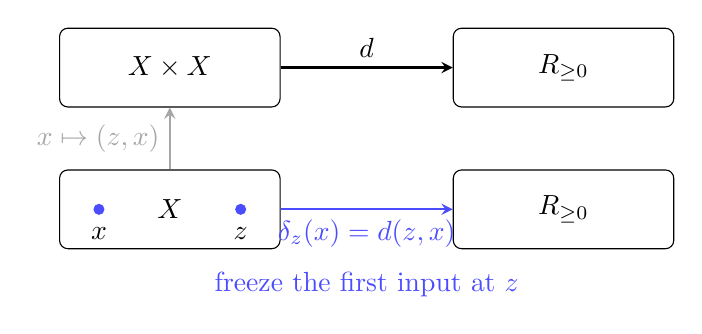
\begin{tikzpicture}[x=1cm,y=1cm,>=stealth]
  \node[draw,rounded corners=3pt,minimum width=2.8cm,minimum height=1cm]
    (product) at (0,1.6) {\(X\times X\)};
  \node[draw,rounded corners=3pt,minimum width=2.8cm,minimum height=1cm]
    (nonneg) at (5,1.6) {\(\mathbb{R}_{\geq 0}\)};
  \draw[->,thick] (product) -- node[above] {\(d\)} (nonneg);

  \node[draw,rounded corners=3pt,minimum width=2.8cm,minimum height=1cm]
    (space) at (0,-0.2) {\(X\)};
  \node[draw,rounded corners=3pt,minimum width=2.8cm,minimum height=1cm]
    (profile) at (5,-0.2) {\(\mathbb{R}_{\geq 0}\)};
  \draw[->,thick,blue!70] (space) -- node[below] {\(\delta_z(x)=d(z,x)\)} (profile);

  \draw[->,gray!70,thick] (space.north) -- node[left] {\(x\mapsto(z,x)\)} (product.south);
  \node[blue!70] at (2.5,-1.15) {freeze the first input at \(z\)};

  \fill[blue!70] (-0.9,-0.2) circle (2pt);
  \node[below=3pt] at (-0.9,-0.2) {\(x\)};
  \fill[blue!70] (0.9,-0.2) circle (2pt);
  \node[below=3pt] at (0.9,-0.2) {\(z\)};
\end{tikzpicture}

\caption{A metric \(d:X\times X\to\mathbb{R}_{\geq 0}\) becomes the point
function \(\delta_z:X\to\mathbb{R}_{\geq 0}\) when the first input is fixed at
\(z\).}
\label{fig:point-function-freezes-metric}
\end{figure}

\begin{definitionbox}{Definition --- Point Function}
\begin{definition}[Point Function]\label{def:metric-point-function}
Let \((X,d)\) be a metric space and let \(z\in X\).  The
\emph{point function at \(z\)} is the function
\[
  \delta_z:X\to\mathbb{R}_{\geq 0},
  \qquad
  \delta_z(x):=d(z,x).
\]
The set of all point functions on \(X\) is denoted by
\[
  \delta(X):=\{\,\delta_z:z\in X\,\}.
\]
\end{definition}
\end{definitionbox}

\LeanFormalizes{def:metric-point-function}{lra-lean}{LRA.VolumeIV.MetricSpaces.Functions.Pointlike}{pointFunction}{statement}
\LeanFormalizes{def:metric-point-function}{lra-lean}{LRA.VolumeIV.MetricSpaces.Functions.Pointlike}{pointFunctions}{statement}

\begin{remark*}[Standard quantified statement]
\[
z\in X
\Longrightarrow
\delta_z:X\to\mathbb{R}_{\geq 0}
\quad\text{and}\quad
\forall x\in X{:}\ \delta_z(x)=d(z,x).
\]
\end{remark*}

\begin{remark*}[Interpretation]
The point function \(\delta_z\) is the distance-from-\(z\) profile.  It turns
the fixed point \(z\) into a one-variable nonnegative real-valued function on
the whole space.
\end{remark*}

\begin{remark*}[Examples]
In \(\mathbb{R}\) with the usual metric \(d(x,y)=|x-y|\), the point function
at \(z\in\mathbb{R}\) is
\[
  \delta_z(x)=d(z,x)=|x-z|.
\]
For example, the point function at \(2\) is
\[
  \delta_2(x)=|x-2|.
\]
It has value \(0\) exactly at \(x=2\), and its graph is the familiar
\(V\)-shape with vertex at \((2,0)\).  Thus the point \(2\) is encoded by the
whole distance profile \(x\mapsto |x-2|\).
\end{remark*}

\begin{dependencies}
\begin{itemize}
  \item \hyperref[def:metric-space]{Definition: Metric Space}
\end{itemize}
\end{dependencies}

\begin{theorembox}{Theorem}
\begin{theorem}[Point Functions Identify Points]
\label{thm:metric-point-functions-identify-points}
Let \((X,d)\) be a metric space.  The map
\[
  X\to\delta(X),
  \qquad
  z\mapsto\delta_z
\]
is a bijection.

\smallskip
\noindent
\hyperref[prf:metric-point-functions-identify-points]{\textit{Go to proof.}}
\end{theorem}
\end{theorembox}

\LeanFormalizes{thm:metric-point-functions-identify-points}{lra-lean}{LRA.VolumeIV.MetricSpaces.Functions.Pointlike}{point_functions_identify_points}{checked}

\begin{remark*}[Standard quantified statement]
\[
z\mapsto\delta_z
\quad\text{is a bijection from }X\text{ onto }\delta(X).
\]
\end{remark*}

\begin{remark*}[Interpretation]
No two different points have the same distance profile.  The zero-distance
law recovers \(z\) from \(\delta_z\), because \(\delta_z(z)=0\) and no other
point has zero distance from \(z\).
\end{remark*}

\begin{remark*}[Exposition]
The statement that
\[
  z\longmapsto\delta_z
\]
is a bijection from \(X\) onto \(\delta(X)\) contains two different levels of
objects.

First, for a fixed point \(z\in X\), the symbol \(\delta_z\) denotes a
function
\[
  \delta_z:X\to\mathbb{R}_{\geq 0},
  \qquad
  \delta_z(x)=d(z,x).
\]
Here \(x\) is the variable input of the function \(\delta_z\).  The value
\(\delta_z(x)\) is a number: the distance from the fixed base point \(z\) to
the point \(x\).

Second, the assignment
\[
  F:X\to\delta(X),
  \qquad
  F(z)=\delta_z,
\]
has a different input and output.  Its input is a point \(z\in X\), but its
output is not a number.  Its output is the entire function \(\delta_z\).
Thus \(F\) sends points of \(X\) to distance-from-that-point functions.

To prove that \(F\) is bijective, it is enough to prove surjectivity and
injectivity.

Surjectivity is built into the definition of the codomain.  By definition,
\[
  \delta(X)=\{\,\delta_z:z\in X\,\}.
\]
Therefore every element of \(\delta(X)\) is already one of the functions
produced by some point \(z\in X\).  So \(F:X\to\delta(X)\) is surjective onto
its declared codomain.

Injectivity is the substantive part.  Suppose \(z_1,z_2\in X\) and
\[
  F(z_1)=F(z_2).
\]
This means
\[
  \delta_{z_1}=\delta_{z_2}
\]
as functions.  Equality of functions means equality at every input, so
\[
  d(z_1,x)=d(z_2,x)
\]
for every \(x\in X\).  Since this holds for every \(x\), choose the particular
input \(x=z_1\).  Then
\[
  d(z_1,z_1)=d(z_2,z_1).
\]
The left-hand side is \(0\), so
\[
  d(z_2,z_1)=0.
\]
By the identity of indiscernibles for a metric, \(z_2=z_1\).  Hence two
points that determine the same point function must be the same point.

Thus \(F\) is surjective because \(\delta(X)\) is defined as its image, and
injective because a metric separates distinct points.  Therefore
\(z\mapsto\delta_z\) is a bijection from \(X\) onto \(\delta(X)\).
\end{remark*}

\begin{dependencies}
\begin{itemize}
  \item \hyperref[def:metric-space]{Definition: Metric Space}
  \item \hyperref[def:metric-point-function]{Definition: Point Function}
\end{itemize}
\end{dependencies}

\begin{theorembox}{Theorem}
\begin{theorem}[Point Function Inequalities]
\label{thm:metric-point-function-inequalities}
Let \((X,d)\) be a nonempty metric space and let \(z\in X\).  Then, for all
\(a,b\in X\),
\[
  \delta_z(b)-\delta_z(a)\leq d(a,b)\leq \delta_z(b)+\delta_z(a),
\]
and
\[
  \delta_z(z)=0.
\]

\smallskip
\noindent
\hyperref[prf:metric-point-function-inequalities]{\textit{Go to proof.}}
\end{theorem}
\end{theorembox}

\LeanFormalizes{thm:metric-point-function-inequalities}{lra-lean}{LRA.VolumeIV.MetricSpaces.Functions.Pointlike}{point_function_inequalities}{checked}
\LeanFormalizes{thm:metric-point-function-inequalities}{lra-lean}{LRA.VolumeIV.MetricSpaces.Functions.Pointlike}{pointFunction_pointlike}{checked}

\begin{remark*}[Standard quantified statement]
\[
\forall a,b\in X{:}\quad
\delta_z(b)-\delta_z(a)\leq d(a,b)\leq \delta_z(b)+\delta_z(a),
\qquad
\delta_z(z)=0.
\]
\end{remark*}

\begin{remark*}[Predicate reading]
\[
\delta_z(b)-\delta_z(a)\leq d(a,b)\leq \delta_z(b)+\delta_z(a)
\]
means that each point function obeys the two-sided distance inequalities
forced by the metric.
\end{remark*}

\begin{remark*}[Interpretation]
Point functions mimic the metric because they are built from the metric.  The
right-hand inequality is the triangle inequality through \(z\), while the
left-hand inequality is the reverse triangle estimate.
\end{remark*}

\begin{dependencies}
\begin{itemize}
  \item \hyperref[def:metric-space]{Definition: Metric Space}
  \item \hyperref[def:metric-point-function]{Definition: Point Function}
\end{itemize}
\end{dependencies}

\begin{definitionbox}{Definition --- Pointlike Function}
\begin{definition}[Pointlike Function]\label{def:metric-pointlike-function}
Let \((X,d)\) be a nonempty metric space.  A function
\[
  u:X\to\mathbb{R}_{\geq 0}
\]
is \emph{pointlike} on \(X\) if, for all \(a,b\in X\),
\[
  u(a)-u(b)\leq d(a,b)\leq u(a)+u(b).
\]
\end{definition}
\end{definitionbox}

\LeanFormalizes{def:metric-pointlike-function}{lra-lean}{LRA.VolumeIV.MetricSpaces.Functions.Pointlike}{Pointlike}{statement}

\begin{remark*}[Standard quantified statement]
\[
\operatorname{IsPointlike}(u,(X,d))
\quad\Longleftrightarrow\quad
u\colon X\to\mathbb{R}_{\geq 0}
\;\land\;
\forall a,b\in X{:}\ u(a)-u(b)\leq d(a,b)\leq u(a)+u(b).
\]
\end{remark*}

\begin{remark*}[Predicate reading]
\[
u\colon X\to\mathbb{R}_{\geq 0}
\quad\text{and}\quad
\operatorname{IsPointlike}(u,(X,d))
\]
means that \(u\) is pointlike with respect to the metric space \((X,d)\).
The predicate depends on the metric space because the inequalities use the
distance function \(d\).
\end{remark*}

\begin{remark*}[Interpretation]
A pointlike function satisfies the inequalities that every point function
satisfies.  It behaves like a distance-from-something profile, even before a
point realizing that profile has been identified.
\end{remark*}

\begin{dependencies}
\begin{itemize}
  \item \hyperref[def:metric-space]{Definition: Metric Space}
  \item \hyperref[thm:metric-point-function-inequalities]{Theorem: Point Function Inequalities}
\end{itemize}
\end{dependencies}

\begin{theorembox}{Theorem}
\begin{theorem}[Pointlike Functions with a Zero Are Point Functions]
\label{thm:metric-pointlike-zero-point-function}
Let \((X,d)\) be a metric space and let \(u:X\to\mathbb{R}_{\geq 0}\).  Then
\(u\in\delta(X)\) if and only if \(u\) is pointlike on \(X\) and
\[
  0\in u(X).
\]
In that case, there is a unique \(w\in X\) such that \(u(w)=0\), and
\[
  u=\delta_w.
\]

\smallskip
\noindent
\hyperref[prf:metric-pointlike-zero-point-function]{\textit{Go to proof.}}
\end{theorem}
\end{theorembox}

\LeanFormalizes{thm:metric-pointlike-zero-point-function}{lra-lean}{LRA.VolumeIV.MetricSpaces.Functions.Pointlike}{pointlike_eq_pointFunction_of_zero}{checked}
\LeanFormalizes{thm:metric-pointlike-zero-point-function}{lra-lean}{LRA.VolumeIV.MetricSpaces.Functions.Pointlike}{pointlike_zero_point_function}{checked}
\LeanFormalizes{thm:metric-pointlike-zero-point-function}{lra-lean}{LRA.VolumeIV.MetricSpaces.Functions.Pointlike}{pointlike_zero_unique}{checked}

\begin{remark*}[Standard quantified statement]
\[
u\in\delta(X)
\quad\Longleftrightarrow\quad
\operatorname{IsPointlike}(u,(X,d))
\;\land\;
0\in u(X).
\]
\end{remark*}

\begin{remark*}[Interpretation]
The zero value anchors a pointlike function to an actual point of \(X\).  Once
\(u(w)=0\), the pointlike inequalities force \(u(a)=d(w,a)\) for every
\(a\in X\), so \(u\) is exactly the point function \(\delta_w\).
\end{remark*}

\begin{dependencies}
\begin{itemize}
  \item \hyperref[def:metric-point-function]{Definition: Point Function}
  \item \hyperref[def:metric-pointlike-function]{Definition: Pointlike Function}
\end{itemize}
\end{dependencies}
